% Eight-page ICRA conference version of phri_combined.tex.
% The journal manuscript and supplementary material remain separate artifacts.
\documentclass[conference]{IEEEtran}

\usepackage{amsmath,amssymb,amsfonts}
\usepackage{amsthm}
\usepackage{graphicx}
\usepackage{booktabs}
\usepackage{bm}
\usepackage{cite}
\usepackage{enumitem}
\usepackage[hidelinks]{hyperref}

\interdisplaylinepenalty=2500
\newtheorem{proposition}{Proposition}
\newtheorem{remark}{Remark}

\newcommand{\Lam}{\Lambda(q)}
\newcommand{\Laminv}{\Lambda^{-1}(q)}
\newcommand{\Fmpc}{F_{\mathrm{mpc}}}
\newcommand{\dhat}{\hat d}
\newcommand{\Nbar}{\bar N}

\setlength{\textfloatsep}{5pt plus 2pt minus 2pt}
\setlength{\floatsep}{4pt plus 2pt minus 2pt}
\setlength{\intextsep}{4pt plus 2pt minus 2pt}
\setlength{\abovecaptionskip}{2pt}
\setlength{\belowcaptionskip}{0pt}
\setlength{\abovedisplayskip}{3pt plus 1pt minus 1pt}
\setlength{\belowdisplayskip}{3pt plus 1pt minus 1pt}

\begin{document}

\title{Compact Offset-Free Interaction-Error MPC with Applied-Torque Constraints for Physical Human--Robot 
Interaction}
\author{\IEEEauthorblockN{Anonymous Authors}}
\maketitle

\begin{abstract}
Reference-holding physical human--robot interaction requires compliant
transient response without retaining a static deflection under sustained
load. We present a compact offset-free model-predictive controller for
torque-controlled manipulators. Operational-space cancellation reduces the
translational tracking error to a double integrator with a
configuration-independent transition matrix. A recursive Kalman filter
estimates the persistent interaction and model mismatch in force coordinates,
and a 30-variable quadratic program predicts the error while constraining the
complete first applied joint-torque command. In a 1\,kHz MuJoCo simulation of
a 7-DOF Franka FR3, adding the disturbance state to an otherwise identical
100\,Hz MPC reduces repeated-step steady-state error from 2.77 to
0.042\,mm. A response-matched impedance baseline reaches 2.59\,mm but briefly
saturates and requires 3.3 times the peak positive joint power; ideal
measured-force cancellation reaches 1.39\,mm. The proposed sensorless
controller therefore isolates a $65.8\times$ offset-rejection benefit in the
tested moving task without increasing peak power.
\end{abstract}

\begin{IEEEkeywords}
Physical human--robot interaction, model predictive control, impedance
control, disturbance estimation, torque constraints.
\end{IEEEkeywords}

\section{Introduction}

Impedance and admittance control provide transparent interaction behavior
\cite{hogan1985impedance,chiaverini1999survey}. Their objectives depend on the
task: in hand guiding, force-induced displacement may be the command, whereas
reference-holding and recovery require a robot to return to a desired motion
after yielding to contact. A finite-stiffness impedance retains the equilibrium
bias $p-p_d=K_d^{-1}F_h$ under a sustained human force $F_h$. Integral action
can remove this bias, but must be coordinated with actuator saturation
\cite{cao2004antiwindup,cao2002antiwindup}.

Predictive interaction control is already well established. Existing work
optimizes interaction dynamics \cite{gold2023mpic}, combines impedance and
constraint optimization \cite{chen2025unified}, learns interaction models
\cite{haninger2023model}, estimates force online \cite{jordana2024force}, or
enforces passivity and safety conditions
\cite{cao2023passive,matschek2023safe}. High-rate nonlinear manipulator MPC is
also possible with tailored computation \cite{kleff2021highfrequency}. Thus
MPC, disturbance estimation, and predictive impedance are not individually
new.

Offset-free MPC commonly augments a nominal model with a constant output or
input disturbance and estimates that state online
\cite{pannocchia2003disturbance}. The choice of disturbance coordinates is
important here. An acceleration disturbance changes with the robot's
configuration through the task inertia, whereas a constant Cartesian load is
approximately constant in force coordinates. We therefore place the
disturbance in the same force channel as the optimizer. This also distinguishes
load rejection from intent inference: the estimated vector includes contact,
unmodelled dynamics, and cancellation error and cannot identify which part was
generated deliberately by a person.

This paper addresses a narrower implementation question: how can these ideas
be connected through a small, auditable interface? Operational-space
cancellation exposes a normalized translational error model. The optimizer
selects a corrective task force, the disturbance estimator uses the same force
coordinates, and the robot-specific realization enters an affine joint-torque
constraint. The contributions are:

\begin{enumerate}[leftmargin=*,itemsep=1pt,topsep=2pt]
\item a constant-transition interaction-error predictor whose input matrix is
scheduled only through the current task inertia;
\item force-domain disturbance augmentation with a centered input cost that
admits the steady balancing input $\Fmpc=-\dhat$; and
\item a first-move applied-torque constraint and a controlled FR3 simulation
comparison against nominal, response-matched, integral, variable-impedance,
and ideal measured-force baselines.
\end{enumerate}

The conference version focuses on the implemented controller and its causal
ablation. Longer proofs, parameter sweeps, and optional barrier/passivity
extensions are not used to support the principal experimental claim.

\subsection{Problem statement and evaluation questions}

Given $p_d(t)$, joint feedback $(q,\dot q)$, and a model
$(M,C,G,J)$, the reference-holding objective is to minimize
$e=p_d-p$ while respecting the physical joint-torque box. No contact-force
measurement is supplied to the proposed controller. We ask three concrete
questions. First, can a 3-D disturbance state remove the sustained-load bias
without changing the nominal MPC tuning? Second, does the comparison remain
meaningful after matching a classical impedance controller to the MPC's
closed-loop response and enforcing the same actuator limits? Third, how does
the flat disturbance prediction degrade under time-varying loads? These
questions determine the ablations and metrics in Section~V.

\section{Interaction-Error Model}

Consider an $n$-DOF torque-controlled manipulator; the experiments use the
Franka FR3 ($n=7$) \cite{franka2023fr3}. Its dynamics are
\begin{equation}
M(q)\ddot q+C(q,\dot q)\dot q+G(q)=\tau+J^\top(q)\mathcal F_h,
\label{eq:eom}
\end{equation}
where $\mathcal F_h$ is positive when the human pushes onto the robot. Let
$J_v\in\mathbb R^{3\times n}$ be the translational Jacobian and
\begin{equation}
\Lambda(q)=\left(J_vM^{-1}J_v^\top\right)^{-1}
\label{eq:lambda}
\end{equation}
the translational operational-space inertia \cite{khatib1987unified}. The
implementation regularizes $\Lambda^{-1}$ by $10^{-6}I$ and operates away
from singularities.

The commanded torque separates feedforward, translation, orientation, and
null-space channels:
\begin{equation}
\tau=\tau_{\rm ff}+J_v^\top\Fmpc+J_\omega^\top F_{\rm ori}
      +\Nbar^\top\tau_{\rm null},
\label{eq:torque}
\end{equation}
where $\Nbar$ is the dynamically consistent projector of the full pose task
\cite{sentis2005synthesis}. Feedforward cancellation uses
\begin{equation}
\tau_{\rm ff}=C\dot q+G+J_v^\top\Lambda\ddot p_d.
\label{eq:feedforward}
\end{equation}
With $e=p_d-p$, the residual translation is
\begin{equation}
\ddot e=-\Lambda^{-1}(q)\Fmpc+d_{\rm acc},
\label{eq:error}
\end{equation}
where $d_{\rm acc}$ collects the projected interaction wrench,
$-\dot J_v\dot q$, orientation-to-translation coupling, friction, and model
error. Hence this is a cancellation-plus-disturbance model, not an assumption
of perfect nonlinear inversion. We use the force-equivalent disturbance
$d=-\Lambda d_{\rm acc}$, which is constant for a constant translational
human force even when $\Lambda(q)$ changes.

For error state $x=[e^\top,\dot e^\top]^\top$ and sample period $\Delta t$,
exact zero-order-hold discretization gives
\begin{equation}
x_{k+1}=A_dx_k+B_d(q_k)(F_{\mathrm{mpc},k}+d_k),
\label{eq:discrete}
\end{equation}
\begin{equation}
A_d=\begin{bmatrix}I&\Delta t I\\0&I\end{bmatrix},\quad
B_d(q)=\begin{bmatrix}-\frac{\Delta t^2}{2}\Lambda^{-1}(q)\\
-\Delta t\Lambda^{-1}(q)\end{bmatrix}.
\label{eq:AB}
\end{equation}
Because the continuous double-integrator matrix is nilpotent, $A_d$ is exact
and configuration independent; only $B_d$ is scheduled. This constant-$A_d$
property applies to the reduced translational predictor, not to the complete
robot dynamics or torque map.

\section{Offset-Free Receding-Horizon Controller}

\subsection{Recursive disturbance estimator}

Augment the force-equivalent disturbance as a random walk:
\begin{equation}
\begin{bmatrix}x_{k+1}\\d_{k+1}\end{bmatrix}=
\begin{bmatrix}A_d&B_d(q_k)\\0&I\end{bmatrix}
\begin{bmatrix}x_k\\d_k\end{bmatrix}+
\begin{bmatrix}B_d(q_k)\\0\end{bmatrix}F_{\mathrm{mpc},k}+
\begin{bmatrix}0\\w_k\end{bmatrix}.
\label{eq:augmented}
\end{equation}
A discrete recursive Kalman filter observes $[e^\top,\dot e^\top]^\top$ from
robot position and velocity feedback and propagates the $9\times9$
covariance at each QP update. Its gain is recomputed rather than frozen.
The random walk tracks constant and slowly varying aggregate loads; it does
not infer human intent or separate human force from model error.

Let $z=[x^\top,d^\top]^\top$, $C_z=[I_6\;0]$, and denote the two matrices in
\eqref{eq:augmented} by $A_z(q_k)$ and $B_z(q_k)$. The implemented recursion is
\begin{subequations}
\begin{align}
\hat z^-_{k+1}&=A_z(q_k)\hat z^+_k+B_z(q_k)F_{\mathrm{mpc},k},\\
P^-_{k+1}&=A_z(q_k)P^+_kA_z^\top(q_k)+Q_z,\\
S_{k+1}&=C_zP^-_{k+1}C_z^\top+R_z,\\
L_{k+1}&=P^-_{k+1}C_z^\top S_{k+1}^{-1},\\
\hat z^+_{k+1}&=\hat z^-_{k+1}+L_{k+1}
 (y_{k+1}-C_z\hat z^-_{k+1}),\label{eq:kf}\\
P^+_{k+1}&=(I-L_{k+1}C_z)P^-_{k+1}.
\end{align}
\end{subequations}
Here $y=[e^\top,\dot e^\top]^\top$, with $p$ from forward kinematics and
$\dot p=J_v\dot q$. The covariance $Q_z$ contains a disturbance random-walk
block $Q_w$; $R_z$ represents the kinematic measurement channel. This filter
uses no extra numerical differentiation of end-effector velocity.

For a frozen nonsingular $B_d$, the disturbance is observable from the
measured error state because it affects $x_{k+1}$ through $B_d$; equivalently,
the first two block rows of the augmented observability matrix contain
$[I_6\;0]$ and $[A_d\;B_d]$. Since $B_d$ has column rank three away from task
singularities, no nonzero disturbance direction is hidden. This establishes
the structural requirement behind the estimator, but does not guarantee a
particular convergence rate under noise or model mismatch.

\subsection{QP and applied-torque constraint}

For horizon $N=10$, stack
$U=[F_{\mathrm{mpc},0}^\top,\ldots,F_{\mathrm{mpc},N-1}^\top]^\top\in\mathbb R^{30}$ and the
predicted errors $X$. With $d_N=\bm 1_N\otimes\dhat$, solve
\begin{subequations}
\begin{align}
\min_U\quad &\frac12X^\top\bar QX+
 \frac12(U+d_N)^\top\bar R(U+d_N),\label{eq:cost}\\
\text{s.t.}\quad &-F_{\max}\le F_{\mathrm{mpc},i}\le F_{\max},\quad i=0{:}N-1,
\label{eq:forcebox}\\
&-\tau_{\max}\le\tau_{\rm base}+J_v^\top F_{\mathrm{mpc},0}
\le\tau_{\max},\label{eq:taubox}
\end{align}
\label{eq:qp}
\end{subequations}
where
$\tau_{\rm base}=\tau_{\rm ff}+J_\omega^\top F_{\rm ori}
+\Nbar^\top\tau_{\rm null}$. The centered effort term in
\eqref{eq:cost}, rather than $\|U\|_{\bar R}^2$, makes the steady balancing
input $U=-d_N$ cost-free. Condensing yields
$H=\Gamma^\top\bar Q\Gamma+\bar R$ and
$h=\Gamma^\top\bar Qx_{\rm free}+\bar R d_N$. The current implementation
tests this identity directly to prevent an absolute-input penalty from
reintroducing an $R$-dependent offset.

For completeness, the condensed prediction used in code is
\begin{equation}
X=\Phi x_k+\Gamma U+D_{\rm bar}\dhat_k,\qquad
D_{\rm bar}=\Gamma(\bm 1_N\otimes I_3),
\label{eq:lifted}
\end{equation}
where the $j$th block row of $\Phi$ is $A_d^j$ and the $(j,i)$ block of
$\Gamma$ is $A_d^{j-1-i}B_d$ for $i<j$. Thus
$x_{\rm free}=\Phi x_k+D_{\rm bar}\dhat_k$ and
\begin{equation}
H=\Gamma^\top\bar Q\Gamma+\bar R,\qquad
h=\Gamma^\top\bar Qx_{\rm free}+\bar R d_N.
\label{eq:condensed}
\end{equation}
Because $\bar R\succ0$, $H\succ0$ and the optimization is a strictly convex
QP. The identity $D_{\rm bar}=\Gamma(\bm 1_N\otimes I_3)$ is also a useful
implementation check: the estimator's force must enter every prediction step
through exactly the same scheduled input map as the commanded force.

\subsection{Relation to a realized impedance}

For fixed $q$, inactive constraints, and $\dhat=0$, the strictly convex QP has
the unique solution
\begin{equation}
U^\star=-H^{-1}\Gamma^\top\bar Q\Phi x_k.
\label{eq:unconstrained}
\end{equation}
If $S_0=[I_3\;0\;\cdots\;0]$ selects the first input block, then
$F_{\mathrm{mpc},0}=S_0U^\star=K_e e+K_{\dot e}\dot e$. The unconstrained
predictive controller is therefore a configuration-dependent linear
impedance whenever the symmetric parts of $K_e$ and $K_{\dot e}$ have the
stiffness and damping sign structure. Importantly, $Q_p$ and $Q_v$ are cost
weights; they are not themselves the realized stiffness and damping. The
realized gains are the finite-horizon Riccati image in
\eqref{eq:unconstrained}.

This relation explains why a nominal 300\,N/m impedance is not automatically a
fair comparator for the tuned MPC. It also identifies what the disturbance
augmentation changes. For a constant load and exact estimate, define
$v=F_{\mathrm{mpc}}+d$. The centered cost penalizes $v$, so the same feedback
acts on the error while the physical command contains the equilibrium
feedforward $F_{\mathrm{mpc}}=-d$. In contrast, an unaugmented finite
stiffness law must retain a nonzero error to produce its balancing force.

Equation~\eqref{eq:taubox} constrains the complete torque that will actually
be applied at the current receding-horizon step, including feedforward,
orientation, and null-space terms. It does not assert horizon-wide torque
feasibility. Because only the first move is applied, the nominal command
satisfies the magnitude limits whenever the QP is feasible. Runtime magnitude
clipping and torque-rate limiting remain final guards. If
$\tau_{\rm base}$ alone exhausts the budget, the released benchmark returns
zero correction on QP failure rather than claiming recursive feasibility.

\begin{proposition}[Frozen-configuration offset rejection]
Fix $q$, assume the augmented pair in \eqref{eq:augmented} is detectable, the
closed loop is stable, the QP is feasible with inactive constraints at steady
state, and the estimator is asymptotically unbiased for a constant $d$. Then
the equilibrium satisfies $e_\infty=0$ and $F_{\mathrm{mpc},\infty}=-d$.
\end{proposition}
\begin{proof}
At equilibrium, \eqref{eq:discrete} requires
$B_d(F_{\mathrm{mpc},\infty}+d)=0$. Away from singularities $B_d$ has full column rank,
so $F_{\mathrm{mpc},\infty}=-d$. With the centered input $V=U+d_N$, the unconstrained
steady solution is $V=0$; positive-definite position weighting and stable
feedback then give $e_\infty=0$.
\end{proof}

This is a frozen-configuration result. Moving-reference performance and active
constraint behavior are evaluated numerically; they are not consequences of
the proposition. For time-varying $d$, flat horizon prediction incurs the
standard bound
\begin{equation}
\|d_{k+i}-\dhat_{k|k}\|\le e_K+L_di\Delta t,
\label{eq:predictionbound}
\end{equation}
when $\|d_k-\dhat_{k|k}\|\le e_K$ and $\|\dot d\|\le L_d$. Only the first
move is applied and the estimate is refreshed at the next solve.

\subsection{Auxiliary channels and implementation scope}

Orientation uses a separate operational-space PD channel. With axis--angle
error $e_R$ extracted from $R_d^\top R$, it applies
\begin{equation}
F_{\rm ori}=-K_{\rm rot}e_R-D_{\rm rot}\omega,\qquad
K_{\rm rot}=20I_3,\quad D_{\rm rot}=6I_3.
\label{eq:orientation}
\end{equation}
This channel is not dynamically decoupled from translation; the resulting
cross-coupling is part of $d_{\rm acc}$ in \eqref{eq:error}.

For the redundant FR3 degree of freedom, define joint clearance
$\phi_i=\min(q_i-q_{\min,i},q_{\max,i}-q_i)$. Within the activation distance
$\delta_i=0.1(q_{\max,i}-q_{\min,i})$, the signed inverse-barrier gradient has
magnitude
\begin{equation}
|g_i(q)|=k_b\left(\frac1{\phi_i}-\frac1{\delta_i}\right),\qquad k_b=50,
\label{eq:softbarrier}
\end{equation}
and points away from the nearer limit. The null-space torque is
$\tau_{\rm null}=-k_{\rm null}(q-q_0)+g(q)-d_{\rm null}\dot q$. Near a task
boundary, the reference is additionally shifted by
\begin{equation}
\delta p=k_{\rm ws}(J_vJ_v^\top+\epsilon_rI)^{-1}J_vg(q),\qquad
\|\delta p\|\le0.06\ {\rm m}.
\label{eq:workspace}
\end{equation}
The circular and waypoint comparisons disable this shift; the boundary test
uses $k_{\rm ws}=5\times10^{-4}$.

The code also contains a one-step control-barrier projection and a
translational energy-tank filter. The direct comparison scripts do not engage
or log those certificates. Moreover, the tank scales only the translational
predictive-force channel and excludes feedforward, orientation, and null-space
power. We therefore make no certified joint-limit or full-port passivity claim
for the experiments below.

The QP runs at 100 or 500\,Hz and the feedforward/realization loop at 1\,kHz.
OSQP \cite{stellato2020osqp} is warm-started and its preallocated matrices are
updated with the current $B_d$, Jacobian, and torque offset. The optimization
dimension is independent of joint count, but deployment still requires the
robot model, full Jacobian, joint limits, and actuator limits.

\section{Real-Time Realization}

The controller is implemented at two rates. At every 1\,kHz physics step, the
robot model, reference acceleration, orientation term, and null-space term are
updated. At a QP tick, the same measured state is used to update the recursive
filter, rebuild the scheduled prediction and affine torque row, and solve for
the first task-force move. That move is held until the next QP tick. This
ordering matters: using an unclipped optimizer output rather than the force
associated with the applied command in \eqref{eq:kf} would give the estimator
a false input whenever a runtime guard activates.

The per-tick sequence is:
\begin{enumerate}[leftmargin=*,itemsep=1pt,topsep=2pt]
\item compute $M,C,G,J_v,J_\omega,\Lambda$ and the measured error $y_k$;
\item predict and correct $(\hat z_k,P_k)$ using the previously applied
task-force correction;
\item form $\Phi,\Gamma,D_{\rm bar}$ from the current $B_d(q_k)$ and construct
$(H,h)$ from \eqref{eq:condensed};
\item add the force box and complete first-move torque row
\eqref{eq:taubox}, warm-start OSQP, and solve;
\item assemble \eqref{eq:torque}, apply the configured runtime guards, and
store the applied correction for the next filter prediction.
\end{enumerate}

Table~\ref{tab:params} records the parameters needed to reproduce the direct
comparison. The optional workspace correction is disabled in the circular and
waypoint controller comparisons and enabled only in the boundary experiment.
The CBF and tank constants are intentionally omitted because those final
filters do not support the headline results.

\begin{table}[t]
\caption{Principal Controller and Estimator Parameters}
\label{tab:params}
\centering
\footnotesize
\setlength{\tabcolsep}{3.0pt}
\begin{tabular}{@{}lll@{}}
\toprule
Quantity & Symbol & Value\\
\midrule
Prediction horizon & $N$ & 10\\
QP period & $\Delta t$ & 10\,ms (2\,ms in C6--C7)\\
Inner realization period & --- & 1\,ms\\
Position / velocity weights & $Q_p,Q_v$ & $2\!\times\!10^4 I_3,\ 50I_3$\\
Terminal scale / effort weight & $\gamma,R$ & $5,\ 10^{-6}I_3$\\
Corrective-force bound & $F_{\max}$ & 150\,N per axis\\
FR3 joint-torque limits & $\tau_{\max}$ & $[87,87,87,87,12,12,12]$\,Nm\\
Disturbance process variance & $Q_w$ & $10I_3$\\
Position / velocity obs. variance & $R_e,R_{\dot e}$ & $10^{-3}I_3,\ 10^{-2}I_3$\\
OSQP tolerances / iteration cap & --- & $10^{-6}$ / 4000\\
\bottomrule
\end{tabular}
\end{table}

Three software checks protect the interface most likely to be implemented
incorrectly. First, the condensed gradient includes $\bar R d_N$; omitting it
changes the intended input-centered cost. Second, the torque bound is applied
to $\tau_{\rm base}+J_v^\top F_{\mathrm{mpc},0}$, not only to the corrective
force. Third, the benchmark logs raw and applied torque separately, using a
$10^{-3}$\,Nm excess threshold so numerical QP tolerances are not mislabeled as
physical saturation.

\section{Simulation Evaluation}

All experiments use the MuJoCo Menagerie FR3
\cite{mujoco_menagerie,todorov2012mujoco} at 1\,kHz with joint-torque limits
$[87,87,87,87,12,12,12]$\,Nm. A 12\,cm XZ circle is traversed in 8\,s while a
15\,N downward step is applied for 3\,s of each cycle. The MPC horizon is
$N=10$, the nominal impedance stiffness is 300\,N/m, and all reported fair
comparators use the same plant and physical torque budget.

\subsection{Estimator and update-rate ablation}

Table~\ref{tab:ablation} separates estimator and update-rate effects. C4 and
C5 have identical horizon, weights, rate, and torque interface; only the
augmented disturbance estimator differs. At 100\,Hz it reduces steady-state
error from 2.77 to 0.042\,mm. Raising the rate mainly reduces the contact
transient in this protocol, while the estimator primarily removes the
constant-load offset; the effects are not claimed to be orthogonal in
general.

\begin{table}[t]
\caption{Controlled MPC Ablation, 15\,N Repeated Step}
\label{tab:ablation}
\centering
\footnotesize
\setlength{\tabcolsep}{3.2pt}
\begin{tabular}{@{}lrrrr@{}}
\toprule
Controller & Rate & Contact RMS & Peak & SS error\\
 & (Hz) & (mm) & (mm) & (mm)\\
\midrule
C4: DI-MPC, no estimator & 100 & 2.20 & 2.92 & 2.77\\
C5: DI-MPC + estimator & 100 & 0.53 & 2.58 & \textbf{0.042}\\
C6: DI-MPC, no estimator & 500 & 0.80 & 1.10 & 1.10\\
C7: DI-MPC + estimator & 500 & \textbf{0.20} & \textbf{0.80} & $<0.05$\\
\bottomrule
\end{tabular}
\end{table}

\subsection{Broad baseline screen}

Before response matching, we screen the controller against four common
interaction behaviors using the nominal 300\,N/m impedance setting. The
admittance controller has a 100\,N/m virtual spring; PI impedance adds an
integral state to the nominal impedance; and predictive variable impedance
uses the disturbance estimate to schedule finite stiffness without cancelling
the load. Table~\ref{tab:broad} reports three cycles and all controllers. It is
included to show behavior across design classes, but comparisons between rows
with different effective stiffness are descriptive rather than causal.

\begin{table}[t]
\caption{Broad Screen on the 12\,cm Circle and 15\,N Step}
\label{tab:broad}
\centering
\footnotesize
\setlength{\tabcolsep}{2.0pt}
\begin{tabular}{@{}lrrrr@{}}
\toprule
Controller & Total RMS & Contact RMS & Peak & SS error\\
 & (mm) & (mm) & (mm) & (mm)\\
\midrule
Impedance, 300\,N/m & 35.6 & 41.1 & 51.8 & 44.8\\
Admittance, 100\,N/m & 113.9 & 174.7 & 210.5 & 186.7\\
PI impedance & 36.2 & 27.4 & 43.7 & 21.4\\
Predictive variable imp. & 12.9 & 4.5 & 7.5 & 4.8\\
C4: DI-MPC 100\,Hz & \textbf{11.4} & 2.2 & 2.9 & 2.8\\
C5: DI-MPC + est. 100\,Hz & \textbf{11.4} & 0.5 & 2.6 & $<0.05$\\
C6: DI-MPC 500\,Hz & 12.8 & 0.8 & 1.1 & 1.1\\
C7: DI-MPC + est. 500\,Hz & 12.6 & \textbf{0.2} & \textbf{0.8} & $<0.05$\\
\bottomrule
\end{tabular}
\end{table}

\begin{figure}[t]
\centering
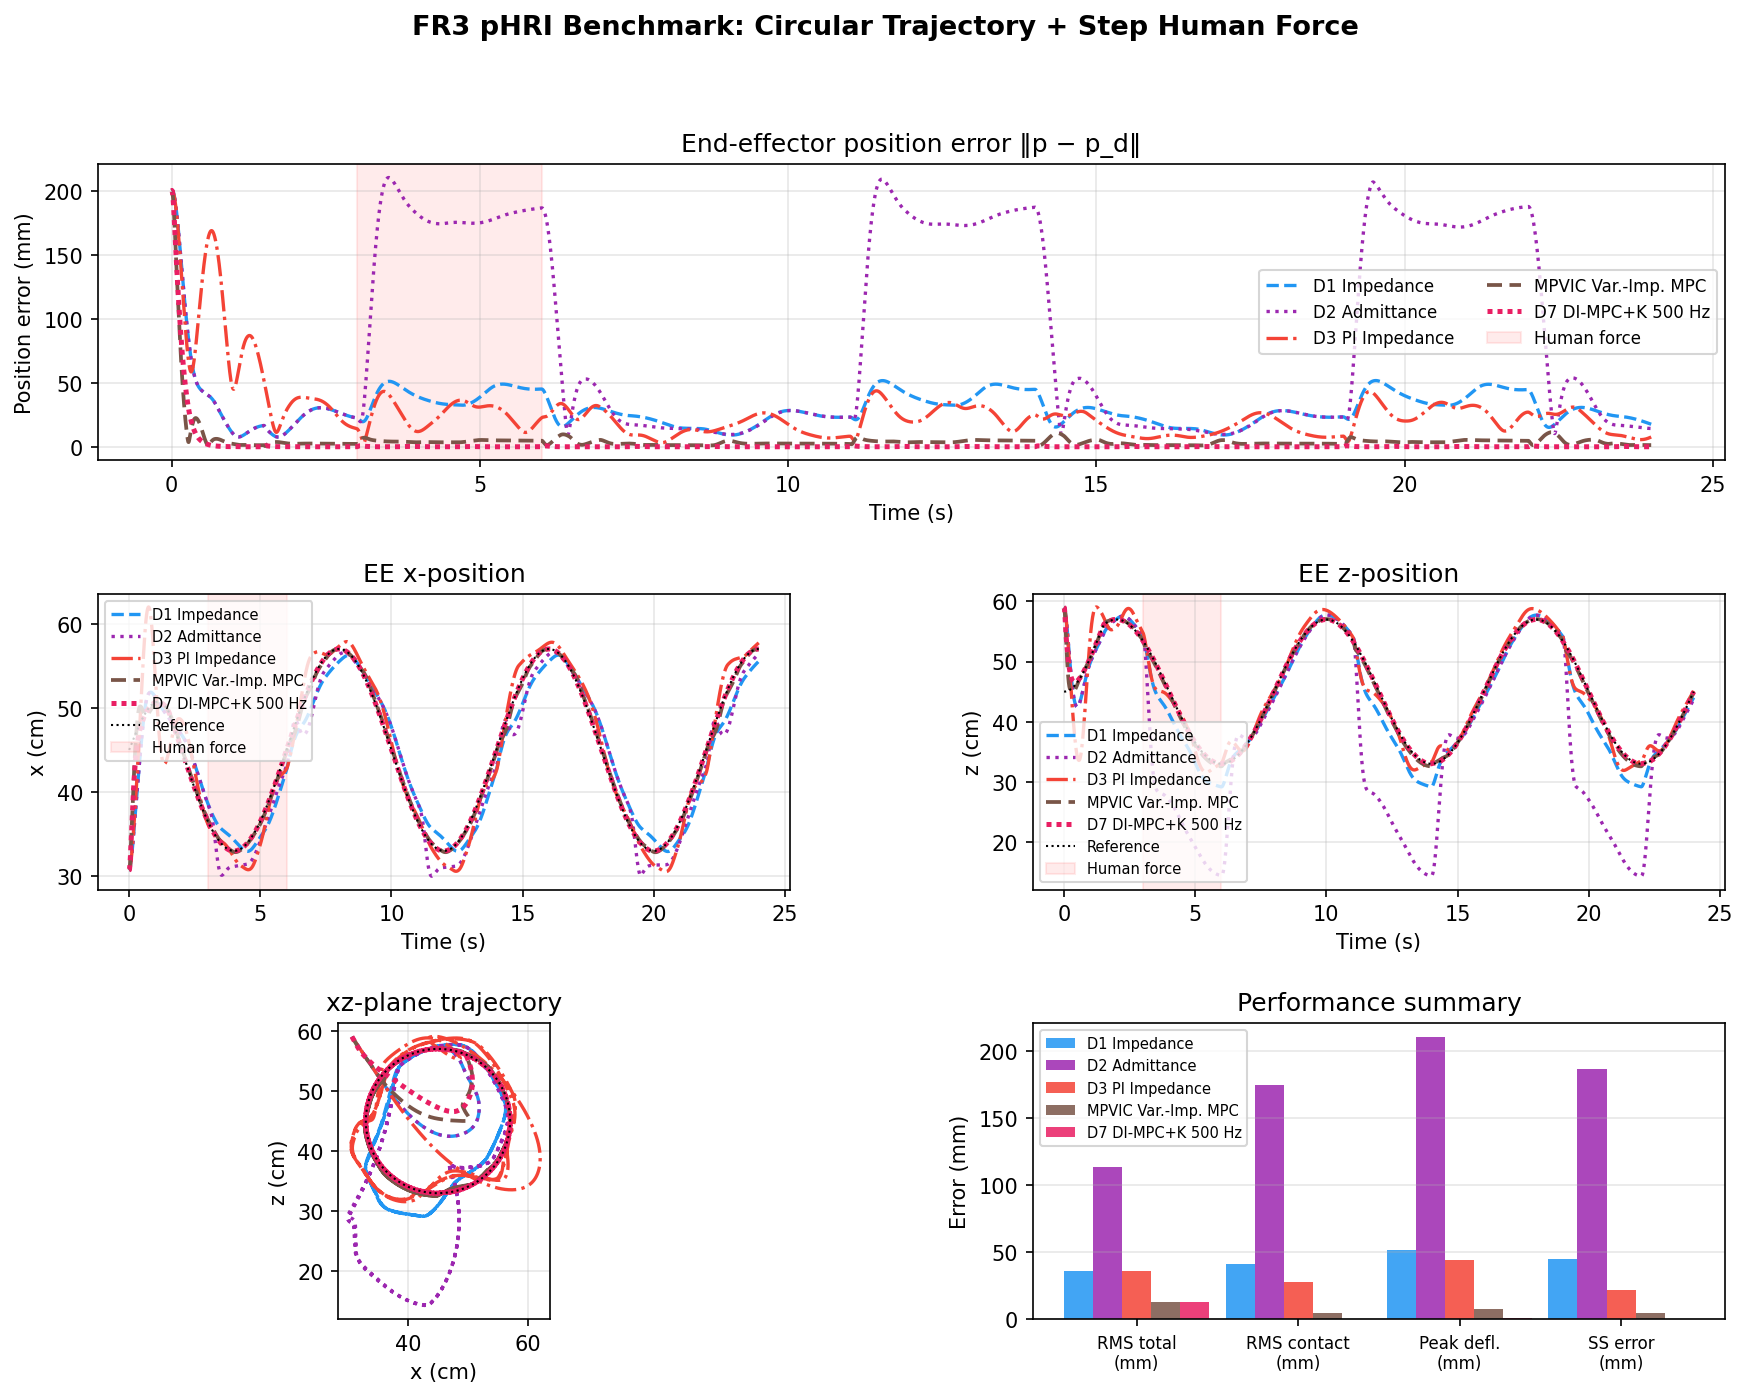
\includegraphics[width=.78\columnwidth]{figures/mpc_comparison_results.png}
\caption{Representative trajectories from the broad screen. The compliant
admittance response is intentional; its large displacement is not a failure
for a guidance task, but it is unsuitable for the reference-holding objective
studied here. The response-matched study below removes the largest stiffness
confound between impedance and MPC.}
\label{fig:broad}
\end{figure}

The broad screen makes two mechanism-level points. The predictive
variable-impedance row improves on reactive finite-stiffness controllers but
retains a 4.8\,mm bias because scheduling stiffness does not provide an
internal model of a constant load. At fixed MPC rate and tuning, C4 versus C5
and C6 versus C7 show the repeatable estimator effect. The exceptionally large
admittance displacement is close to the $15/100=150$\,mm equilibrium expected
from its virtual spring; it reflects its chosen yielding behavior. We do not
use these unmatched rows to claim general superiority.

\subsection{Response-matched fair comparison}

The nominal 300\,N/m impedance is intentionally compliant, so its comparison
with C4 is gain-confounded. A separate calibration estimates C4's equilibrium
stiffness as 5441\,N/m, then searches stiffness scales
$(0.8,1.0,1.2)$ and damping ratios $(0.7,1.0,1.3)$ on one cycle. It selects
5441\,N/m and $\zeta=1.3$. A torque-aware PI baseline is tuned independently
over nine integral-gain/limit pairs. We also provide the matched impedance
with ideal simulated-force cancellation filtered at 50\,ms; this is a
favorable sensor-based comparator, not a reproduction of a particular
published controller. Metrics in Table~\ref{tab:fair} use three held-out
cycles.

\begin{table}[t]
\caption{Fair Comparison Under a Common Actuator Budget}
\label{tab:fair}
\centering
\footnotesize
\setlength{\tabcolsep}{1.4pt}
\begin{tabular}{@{}lrrrr@{}}
\toprule
Controller & Contact & SS & Saturated & Peak $P^+$\\
 & RMS (mm) & (mm) & samples (\%) & (W)\\
\midrule
Nominal impedance & 41.07 & 44.82 & 0 & 22.5\\
Response-matched impedance & 2.38 & 2.59 & 0.45 & 378.2\\
Tuned anti-windup PI & 27.10 & 20.38 & 0 & 58.3\\
Matched imp. + force FF & 1.40 & 1.39 & 0.45 & 378.2\\
C4: DI-MPC 100\,Hz & 2.20 & 2.77 & 0 & 113.2\\
C5: DI-MPC + est. 100\,Hz & \textbf{0.53} & \textbf{0.042} & 0 & 113.1\\
\bottomrule
\end{tabular}
\end{table}

\begin{figure}[t]
\centering
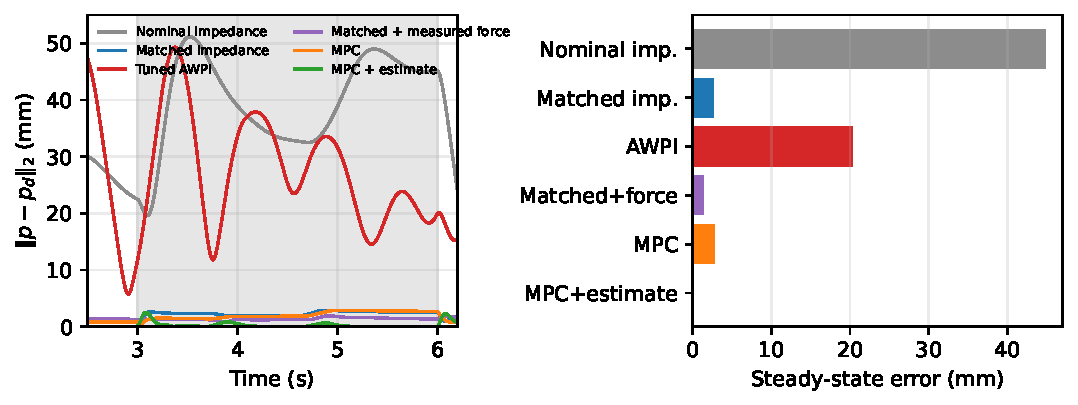
\includegraphics[width=\columnwidth]{figures/fair_offset_free_comparison.pdf}
\caption{Held-out fair comparison. Response matching closes the nominal
impedance/C4 steady-state gap. The controlled C4--C5 pair isolates the
disturbance augmentation; ideal measured-force feedforward also reduces the
load-axis bias but retains the matched impedance's saturation and power cost.}
\label{fig:fair}
\end{figure}

The response-matched impedance and C4 have similar steady-state errors (2.59
and 2.77\,mm), so the nominal impedance/C4 ratio is not an architectural
result. Their resource use differs: the matched impedance reaches 378.2\,W
peak positive joint power and exceeds a physical torque limit in 0.45\% of
samples, compared with 113.2\,W and no thresholded saturation for C4. C4 and
C5 each complete 2400 QP solves without failure; their maximum raw limit
excesses are below $2\times10^{-5}$\,Nm, beneath the $10^{-3}$\,Nm saturation
threshold. Adding the estimator reduces steady-state error by $65.8\times$
without increasing peak power. Ideal measured-force cancellation confirms
that constant-load rejection is not unique to MPC; C5's distinction in this
test is achieving 0.042\,mm without a force measurement.

\subsection{Waypoint generalization}

A second task checks whether the conclusion is specific to a periodic circle.
The end effector visits three waypoints forming a triangle. At each waypoint,
a 15\,N push in a different direction begins 0.8\,s after arrival and lasts
2\,s; the robot must then dwell within 35\,mm of the target for 1\,s. All
controllers reach all three waypoints. Table~\ref{tab:waypoints} repeats the
controlled 100\,Hz estimator ablation: contact RMS falls from 2.2 to 0.6\,mm
when the disturbance state is enabled. At 500\,Hz, estimation and faster
updates combine to reach 0.2\,mm contact RMS and 0.8\,mm peak error.

\begin{table}[t]
\caption{Three-Waypoint Hold Under Directionally Varied Pushes}
\label{tab:waypoints}
\centering
\footnotesize
\setlength{\tabcolsep}{1.6pt}
\begin{tabular}{@{}lrrrr@{}}
\toprule
Controller & Waypoints & Free RMS & Contact RMS & Peak\\
 & reached & (mm) & (mm) & (mm)\\
\midrule
Stiff impedance & 3/3 & 63.6 & 41.4 & 47.1\\
Predictive variable imp. & 3/3 & 51.2 & 5.0 & 6.0\\
C4: DI-MPC 100\,Hz & 3/3 & 47.9 & 2.2 & 2.6\\
C5: DI-MPC + est. 100\,Hz & 3/3 & 47.9 & 0.6 & 2.4\\
C6: DI-MPC 500\,Hz & 3/3 & 51.9 & 0.8 & 1.0\\
C7: DI-MPC + est. 500\,Hz & 3/3 & 51.4 & \textbf{0.2} & \textbf{0.8}\\
\bottomrule
\end{tabular}
\end{table}

The predictive variable-impedance comparator rolls out the same horizon and
uses $\dhat$ only to choose a stiffness from
$\{200,400,800,1500,3000\}$\,N/m; it does not subtract the estimated load.
It is an in-house scheduler in the family of predictive variable-impedance
methods \cite{liu2025model,roveda2019optimal}, not a reproduction of a
published implementation. Its 5.0\,mm result
therefore supports only the mechanism-level observation that adapting a finite
stiffness leaves a load-dependent offset. The large free-motion errors across
methods include waypoint travel and are not a measure of contact regulation.

The moving-reference behavior is also checked on four circle planes without
plane-specific retuning (Table~\ref{tab:planes}). C5 remains below 0.35\,mm
free-space RMS on every plane. The much larger nominal-impedance errors again
mix architecture with its deliberately compliant 300\,N/m gain, so the table
is evidence of directional consistency of the scheduled operational-space
model, not a fair performance ratio.

\begin{table}[t]
\caption{Free-Space Circle Generalization, $R=12$\,cm, $T=8$\,s}
\label{tab:planes}
\centering
\footnotesize
\setlength{\tabcolsep}{3.5pt}
\begin{tabular}{@{}lrr@{}}
\toprule
Circle plane & Nominal impedance RMS & C5 RMS\\
 & (mm) & (mm)\\
\midrule
XZ sagittal & 23.54 & 0.24\\
XY horizontal & 25.06 & 0.33\\
YZ frontal & 16.25 & 0.20\\
Tilted XZ-to-XY & 25.07 & 0.31\\
\bottomrule
\end{tabular}
\end{table}

\subsection{Time-varying interaction and horizon validity}

The random-walk model predicts $d$ as constant over the short horizon. We test
that approximation at a static target under
$F_z=-12\sin(2\pi f t)$\,N for $f\in\{0,0.1,0.2,0.4,0.8\}$\,Hz. From the
simulator dynamics and the applied torque-limited correction, the aggregate
ground truth is reconstructed as
\begin{equation}
d_{{\rm acc},k}=\ddot e_k+\Lambda^{-1}(q_k)F_{\mathrm{mpc},k},\qquad
d_k=-\Lambda(q_k)d_{{\rm acc},k}.
\label{eq:dgroundtruth}
\end{equation}
For prediction origins fully inside the settled force window, define
$e_K={\rm RMS}_k\|d_k-\dhat_{k|k}\|$ and
$\varepsilon_i={\rm RMS}_k\|d_{k+i}-\dhat_{k|k}\|$. The empirical rate
$L_{d,{\rm emp}}$ is the maximum first difference of the reconstructed
aggregate disturbance, not merely the derivative of the injected sinusoid.

\begin{table}[t]
\caption{Ground-Truth Disturbance Prediction, C5 at 100\,Hz}
\label{tab:timevarying}
\centering
\footnotesize
\setlength{\tabcolsep}{2.4pt}
\begin{tabular}{@{}rrrrrr@{}}
\toprule
$f$ & $L_{d,{\rm emp}}$ & $e_K$ & $\varepsilon_1$ & $\varepsilon_N$ & Track RMS\\
(Hz) & (N/s) & (N) & (N) & (N) & (mm)\\
\midrule
0.0 & 0.51 & 2.20 & 2.20 & 2.20 & 0.08\\
0.1 & 7.57 & 0.88 & 0.90 & 1.13 & 0.12\\
0.2 & 15.13 & 2.45 & 2.50 & 3.08 & 0.26\\
0.4 & 30.44 & 4.51 & 4.62 & 5.94 & 0.54\\
0.8 & 61.45 & 5.07 & 5.36 & 8.38 & 1.04\\
\bottomrule
\end{tabular}
\end{table}

For all five rows, the measured $N$-step error is below
$e_K+L_{d,{\rm emp}}N\Delta t$ (2.25, 1.64, 3.97, 7.55, and 11.22\,N,
respectively), consistent with \eqref{eq:predictionbound}. Prediction and
tracking errors increase with disturbance rate: tracking stays below 0.6\,mm
through 0.4\,Hz and reaches 1.04\,mm at 0.8\,Hz. The nonzero constant-row
$e_K$ is mainly estimator fluctuation: its mean error-vector norm is 0.74\,N,
whereas its zero-mean fluctuation RMS is 2.07\,N. This experiment checks the
finite-horizon arithmetic for the simulator protocol; it is not a robustness
bound for unmodelled contact, delay, or hardware sensing.

\subsection{Force magnitude and shape}

The circular experiment is repeated with sustained loads from 5 to 25\,N to
check the operating range of the offset claim (Table~\ref{tab:forcesweep}).
For C7, steady-state deflection remains approximately 0.021\,mm throughout the
tested unsaturated range, whereas first-contact peak error increases from 0.29
to 1.27\,mm. The estimator cancels a constant force after convergence, but it
cannot cancel an unseen step at its first sample; this separates steady-state
offset rejection from transient compliance.

\begin{table}[t]
\caption{Sustained-Force Sweep: Steady-State / Peak Error (mm)}
\label{tab:forcesweep}
\centering
\footnotesize
\setlength{\tabcolsep}{3.0pt}
\begin{tabular}{@{}lrrrrr@{}}
\toprule
Applied load (N) & 5 & 10 & 15 & 20 & 25\\
\midrule
Nominal impedance, SS & 26.9 & 33.7 & 45.0 & 58.5 & 73.1\\
Nominal impedance, peak & 28.4 & 37.0 & 51.2 & 70.1 & 88.9\\
C7, SS & 0.021 & 0.021 & 0.021 & 0.021 & 0.021\\
C7, peak & 0.29 & 0.50 & 0.76 & 1.02 & 1.27\\
\bottomrule
\end{tabular}
\end{table}

At 15\,N, changing the force profile from a step to a linear ramp lowers C7
contact RMS from 0.151 to 0.096\,mm and peak error from 0.759 to 0.286\,mm. A
1\,Hz sinusoid raises contact RMS to 0.402\,mm while peak error remains
0.601\,mm. These results agree with the direct prediction study: smoother
onset reduces the unobserved transient, while a persistent time-varying load
exposes the bandwidth limit of the random-walk estimator. They do not imply
amplitude-independent performance after the 150\,N force box or joint-torque
limits become active.

\subsection{Boundary and robustness checks}

The 20\,cm boundary circle deliberately exercises the soft null-space barrier
and workspace projection, not the final CBF. Nominal impedance reaches a
fractional joint margin of 0.049 and crosses the chosen 5\% threshold; C5
maintains 0.083 at both 100 and 30\,Hz, with 13.33 and 11.76\,mm tracking RMSE.
This is empirical avoidance under the stated trajectory, not forward-invariant
safety certification.

\begin{figure}[t]
\centering
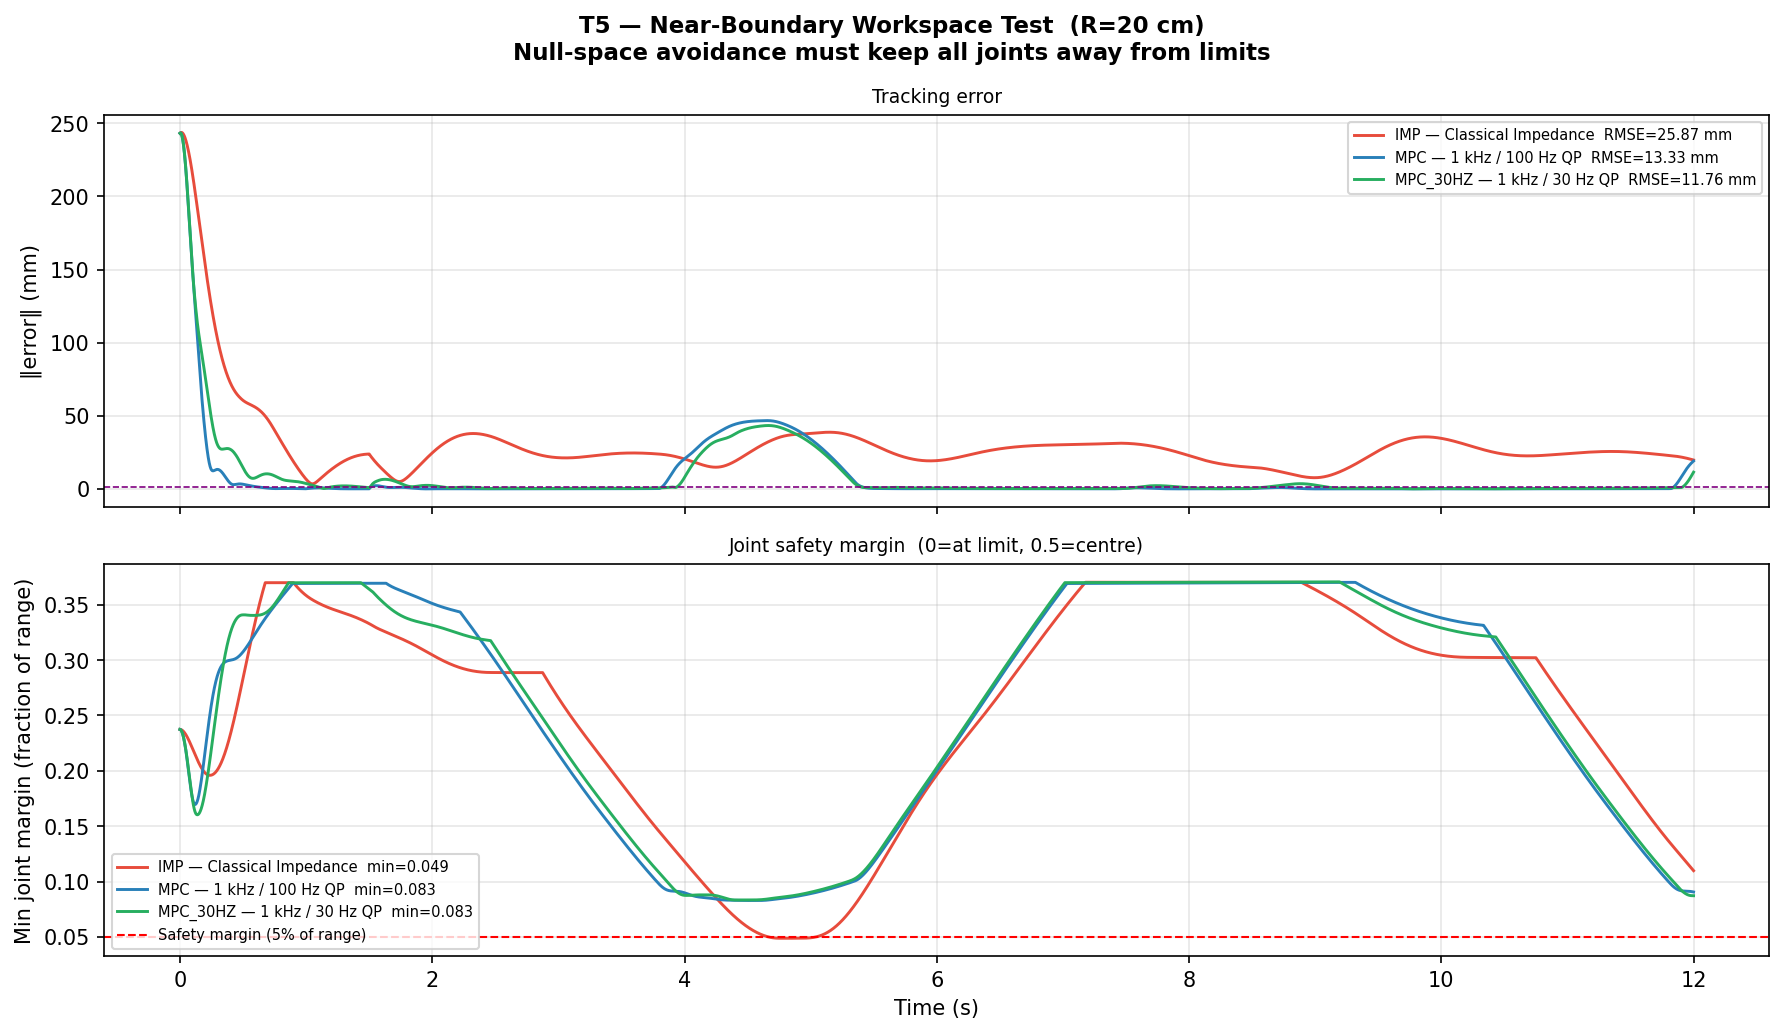
\includegraphics[width=.78\columnwidth]{figures/trajectory_boundary.png}
\caption{Boundary-circle trajectories. The workspace correction trades
tracking accuracy for clearance: the nominal impedance crosses the selected
5\% fractional margin (minimum 0.049), whereas C5 maintains 0.083 in this
test. The plotted result exercises the soft mechanisms in
\eqref{eq:softbarrier}--\eqref{eq:workspace}, not the optional CBF.}
\label{fig:boundary}
\end{figure}

\begin{table}[t]
\caption{C5 Robustness Checks (100\,Hz QP)}
\label{tab:robust}
\centering
\footnotesize
\setlength{\tabcolsep}{2.0pt}
\begin{tabular}{@{}lcccc@{}}
\toprule
Position noise $1\sigma$ (mm) & 0 & 1 & 2 & 5\\
10\,N-step SS error (mm) & 0.08 & $0.19\pm.03$ & $0.37\pm.04$ & $0.89\pm.07$\\
\midrule
Controller inertia error & 0\% & +10\% & +20\% & +30\%\\
Circle RMSE, estimator on (mm) & 0.24 & 0.24 & 0.23 & 0.23\\
Circle RMSE, estimator off (mm) & 0.94 & 0.86 & 0.79 & 0.73\\
\bottomrule
\end{tabular}
\end{table}

Position-noise results average five seeds and model only end-effector position
noise; velocity noise, delay, and force-sensor noise are absent. The inertia
test perturbs only the controller's feedforward model while the plant remains
unchanged. These tests show numerical tolerance over the selected ranges, not
robust-stability guarantees.

\subsection{Loss of corrective authority}

In the standard realization, the QP output is the entire translational
feedback term. If its force box is tightened toward zero, the commanded
translation channel approaches feedforward-only cancellation and retains no
restoring stiffness. This is a meaningful deployment failure mode even though
it is outside the nominal $F_{\max}=150$\,N benchmark. We therefore test an
optional architecture, C8, that places a fixed damped backbone outside the
optimizer,
\begin{equation}
F_{\rm bb}=K_{\rm bb}e+D_{\rm bb}\dot e,\qquad K_{\rm bb}=300I_3\ {\rm N/m},
\label{eq:backbone}
\end{equation}
and lets the QP choose only an additive bounded correction. The full command
$F_{\rm bb}+F_{\rm mpc}$ is included in the torque-feasibility rows. Unlike the
default controller, C8 repeats a frozen-current-configuration torque row at
every horizon step. This is a local realizability approximation, not an exact
future joint-space rollout.

\begin{table}[t]
\caption{Corrective-Authority Stress Test: Contact RMS / Peak (mm)}
\label{tab:authority}
\centering
\footnotesize
\setlength{\tabcolsep}{2.8pt}
\begin{tabular}{@{}lrrrrr@{}}
\toprule
$F_{\max}$ (N) & 150 & 20 & 5 & 1 & 0\\
\midrule
C7 RMS & 0.15 & 0.15 & 317.7 & 416.0 & 430.0\\
C7 peak & 0.77 & 0.76 & 412.2 & 554.2 & 565.9\\
C8 RMS & 0.15 & 0.15 & 41.3 & 69.8 & 78.6\\
C8 peak & 0.77 & 0.76 & 53.7 & 95.9 & 109.4\\
\bottomrule
\end{tabular}
\end{table}

At 150 and 20\,N, C8 matches C7 to the reported precision; the backbone does
not cost nominal performance because it replaces force that the unconstrained
QP would otherwise generate. At 5\,N and below, both controllers degrade
severely, but C8's retained stiffness reduces contact RMS by 5.5--7.7 times
over this 24\,s protocol. At $F_{\max}=0$, C8 still has 78.6\,mm contact RMS:
the backbone improves graceful degradation but cannot reproduce offset-free
control without additive correction. This finite-duration stress test is not
a boundedness, recursive-feasibility, or actuator-fault guarantee. It does,
however, expose a practical distinction between limiting an optional
predictive correction and limiting the controller's entire restoring action.

\section{Discussion and Conclusion}

The proposed interface separates a behavior-coordinate request from its
robot-specific torque realization. Operational-space cancellation gives a
constant-$A_d$ error predictor; force-domain augmentation aligns the estimate,
horizon model, and balancing input; and the affine first-move constraint acts
on the complete applied torque. The C4--C5 ablation attributes a $65.8\times$
steady-state improvement to disturbance augmentation under identical MPC
tuning. Response matching also shows that much of the nominal
impedance-versus-MPC gap is simply stiffness, while ideal force cancellation
confirms that offset rejection is not unique to predictive control.

The evidence remains limited to torque-controlled FR3 simulation. The
predictor lumps human force and model error, assumes accurate position and
velocity feedback, and provides a frozen-configuration offset result. The
boundary test is not a CBF certificate, and the optional energy tank does not
establish full-port passivity. Hardware evaluation should compare against a
canonical predictive interaction controller under shared tuning while logging
force estimates, applied torque, solver status, safety-filter slack, and energy
state.

\IEEEtriggeratref{10}
\bibliographystyle{IEEEtran}
\bibliography{references}

\end{document}
